\chapter{Deep Learning and Machine Learning}

\section{Introduction}
\label{sec:intro}
Artificial intelligence (AI) has become indispensable in medical imaging, offering tools that can assist—and in some cases outperform—radiologists in detecting and characterizing pathologies. In the context of brain tumors, AI-driven methods enable rapid and accurate identification of tumor boundaries and grading, directly impacting treatment planning and patient outcomes.

In this chapter,


\section{What is Artificial Intelligence?}

Artificial Intelligence (\glsxtrshort{ai}) is a multidisciplinary field focused on developing machines and computer programs capable of performing tasks that typically require human intelligence, such as visual perception, reasoning, decision making, and language understanding. According to \cite{sciencedirect_ai_overview}, AI is defined as:

\begin{quotation}
  "the science and engineering of creating intelligent machines, particularly intelligent computer programs that can perform tasks requiring human intelligence, such as visual perception, decision making, and language translation."
\end{quotation}

In other words, AI includes both the study of human cognition—how people perceive, learn, reason, and decide—and the development of algorithms and systems that can perform tasks requiring "intelligence," such as visual recognition or decision making. While some AI techniques draw inspiration from biological processes (e.g. neural networks), the field also embraces purely mathematical and statistical methods.

\begin{figure}[H]
  \centering
  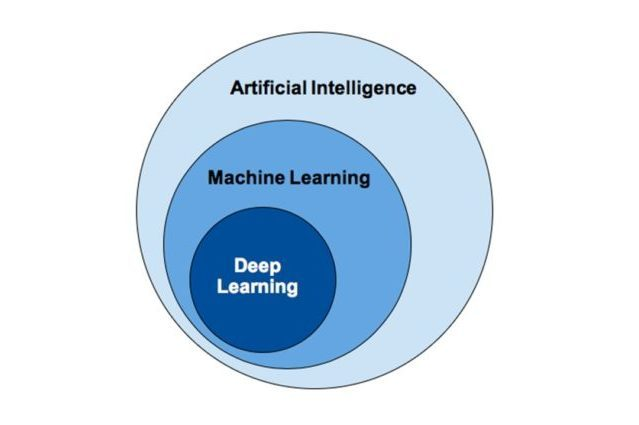
\includegraphics[width=0.6\textwidth]{Images/Chapter1/ai.jpg}
  \caption{Differences between AI, machine learning, and deep learning. \cite{thakkar2020aivsmlvsdl}}
  \label{fig:ai}
\end{figure}

\section{Machine Learning}
\label{sec:ml}
Machine learning (\glsxtrshort{ml}) has emerged as a crucial area of study for organizations aiming to harness data resources and gain deeper insights into their operations. Unlike traditional programming methods, where explicit instructions are coded, machine learning enables systems to learn directly from data. In the medical imaging field, ML techniques offer powerful ways to analyze complex MRI data, supporting more accurate and efficient diagnostic processes. However, machine learning is a complex process that involves using diverse algorithms to iteratively learn from data, refine data representations, and make predictions. By feeding training data into these algorithms, increasingly accurate models can be developed. These machine learning models represent the knowledge acquired by algorithms during the training phase \cite{hurwitz2018mlfd}.

\begin{figure}[H]
  \centering
  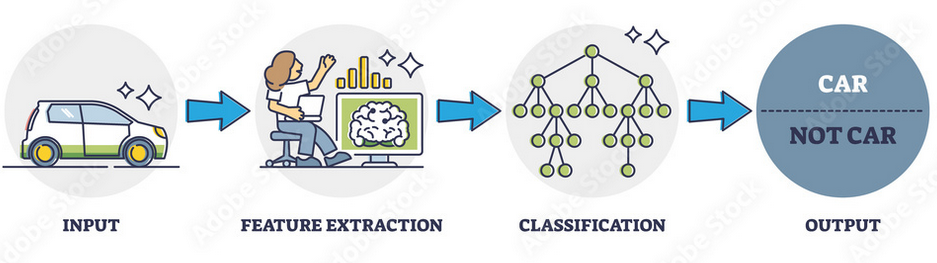
\includegraphics[width=0.8\textwidth]{Images/Chapter1/ml.png}
  \caption{Illustration of the Machine Learning Process \cite{alltius2025deeplearning}}
  \label{fig:ml}
\end{figure}


\subsection{Why Machine Learning?}
\label{sec:why_ml}
Machine learning offers several compelling advantages that have driven its adoption in medical imaging and other fields:

\begin{itemize}
  \item \textbf{Pattern Recognition in Complex Data}: Machine learning excels at discovering patterns in high-dimensional data that may be imperceptible to human observers. For medical imaging, this means identifying subtle tissue abnormalities or correlations that might otherwise be missed.

  \item \textbf{Automation of Repetitive Tasks}: ML algorithms can automate time-consuming aspects of image analysis, freeing radiologists to focus on interpretation and clinical decision-making rather than routine measurements or screenings.

  \item \textbf{Quantitative Assessment}: Unlike qualitative human evaluations that may vary between observers, machine learning provides consistent, quantitative measurements of disease characteristics, potentially reducing inter-observer variability.

  \item \textbf{Integration of Multimodal Data}: Modern ML methods can combine information from multiple imaging modalities (MRI, CT, PET) along with clinical data to provide more comprehensive analysis than would be possible with any single data source.

  \item \textbf{Predictive Capabilities}: Beyond current state assessment, machine learning can predict disease progression or treatment response based on patterns learned from large datasets of prior patients.

  \item \textbf{Personalized Medicine}: ML algorithms can identify subgroups of patients with similar characteristics or disease presentations, enabling more tailored treatment approaches.

  \item \textbf{Continuous Learning}: Machine learning systems can be designed to improve over time as they process more data, unlike traditional rule-based systems that remain static unless manually updated.

  \item \textbf{Cost-Effectiveness}: By improving diagnostic accuracy and efficiency, machine learning can reduce unnecessary tests, treatments, and hospitalizations, potentially lowering healthcare costs.
\end{itemize}

% \subsection{Machine Learning Application Examples}
% \label{sec:ml_applications}
% Machine learning has been successfully applied across numerous domains, with far-reaching impacts in areas such as computer vision, natural language processing, and recommender systems:

% \begin{itemize}
%   \item \textbf{Tumor Detection and Classification}: ML algorithms can detect and classify brain tumors, lung nodules, and other cancerous lesions from imaging data \cite{wang2019machine}.
%   \item \textbf{Disease Progression Monitoring}: Tracking changes in disease markers over time, such as multiple sclerosis lesion load or Alzheimer's-related brain atrophy \cite{mortaheb2019machine}.
%   \item \textbf{Radiomics}: Extracting quantitative features from medical images to improve diagnostic and prognostic accuracy \cite{lambin2012radiomics}.
%   \item \textbf{Resource Allocation}: Predicting hospital readmissions or length of stay to optimize resource allocation \cite{futoma2015comparison}.
%   \item \textbf{Algorithmic Trading}: Making trading decisions based on market data analysis \cite{treleaven2013algorithmic}.
%   \item \textbf{Recommendation Systems}: Suggesting products or content based on user preferences and behavior \cite{ricci2011introduction}.
%   \item \textbf{Churn Prediction}: Identifying customers likely to discontinue services \cite{verbeke2012building}.
%   \item \textbf{Supply Chain Optimization}: Predicting demand and optimizing inventory management \cite{carbonneau2008application}.
%   \item \textbf{Resource Management}: Optimizing water and energy resource allocation \cite{wu2014real}.
% \end{itemize}

\subsection{Different Techniques and Algorithms in Machine Learning}
\label{sec:ml_techniques}
Machine learning encompasses a diverse array of techniques and algorithms, each with unique strengths for specific types of problems, we mention some of them:

\textbf{Classification Algorithms}:
\begin{itemize}
  \item \textbf{Support Vector Machines (SVMs)}: Algorithms that find the optimal hyperplane to separate classes in high-dimensional space \cite{cortes1995support}.
  \item \textbf{Random Forests}: Ensemble learning methods that construct multiple decision trees and output the class that is the mode of the classes of individual trees \cite{breiman2001random}.
  \item \textbf{Naive Bayes}: Probabilistic classifiers based on applying Bayes' theorem with strong independence assumptions \cite{rish2001empirical}.
  \item \textbf{k-Nearest Neighbors (k-NN)}: Instance-based learning where an object is classified by a majority vote of its neighbors \cite{cover1967nearest}.
\end{itemize}

\textbf{Regression Algorithms}:
\begin{itemize}
  \item \textbf{Linear Regression}: Modeling the relationship between a dependent variable and independent variables using a linear approach \cite{montgomery2021introduction}.
  \item \textbf{Lasso Regression}: Linear regression with L1 regularization that can perform feature selection \cite{tibshirani1996regression}.
  \item \textbf{Gaussian Process Regression}: A non-parametric approach using Gaussian processes for modeling \cite{rasmussen2003gaussian}.
\end{itemize}

\textbf{Clustering Algorithms}:
\begin{itemize}
  \item \textbf{K-Means}: Partitioning observations into k clusters based on the nearest mean \cite{macqueen1967some}.
  \item \textbf{Hierarchical Clustering}: Building a hierarchy of clusters either through agglomerative or divisive approaches \cite{johnson1967hierarchical}.
\end{itemize}

\subsection{Machine Learning approachs}
Machine learning algorithms can be categorized into three main categories: supervised learning, unsupervised learning, and reinforcement learning. In the following sections, we will explore each of these categories in more detail, highlighting their strengths and weaknesses, and providing examples of how they are used in medical imaging analysis.
\subsubsection{Supervised Learning}
In supervised learning, the algorithm learns from labeled training data, where each data point is associated with a corresponding label or target value as depicted in Figure \ref{fig:superml}. Examples of supervised learning algorithms include linear regression , decision trees , random forests , support vector machines.

\begin{figure}[H]
  \centering
  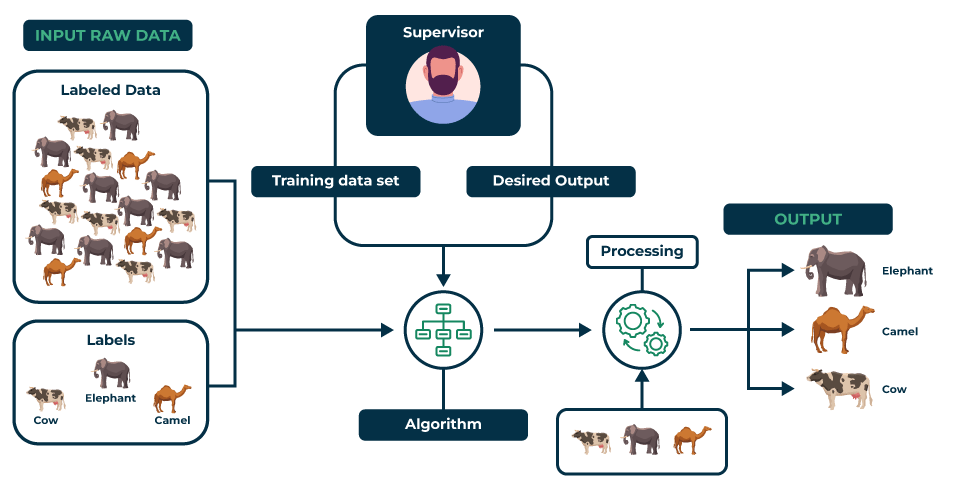
\includegraphics[width=0.8\textwidth]{Images/Chapter1/superml.png}
  \caption{Illustration of the Supervised learning process \cite{geeksforgeeks2025supervised}}
  \label{fig:superml}
\end{figure}

\subsubsection{Unsupervised Learning}
Unsupervised learning deals with unlabeled data, where the algorithm learns to find patterns or
structure in the data without any specific guidance. Such as k-means and hierarchical
clustering, and dimensionality reduction techniques, such as principal component analysis
and t-distributed stochastic neighbor embedding,  Figure \ref{fig:unsuperml}
\begin{figure}[H]
  \centering
  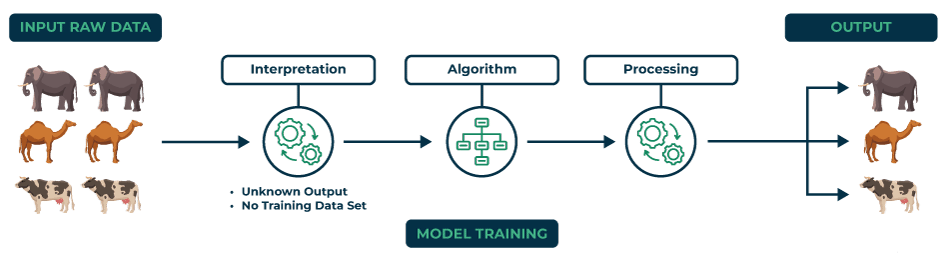
\includegraphics[width=0.8\textwidth]{Images/Chapter1/unsuperml.png}
  \caption{Illustration of the Unsupervised learning process \cite{geeksforgeeks2025supervised} }
  \label{fig:unsuperml}
\end{figure}

\subsubsection{Reinforcement Learning}
Reinforcement learning is a type of machine learning where an agent learns to make decisions by interacting with an environment. The agent receives feedback in the form of rewards or penalties based on its actions, allowing it to learn optimal strategies over time. This approach is often used in robotics, game playing, and autonomous systems. Figure \ref{fig:reinforcement} illustrates the reinforcement learning process.
\begin{figure}[H]
  \centering
  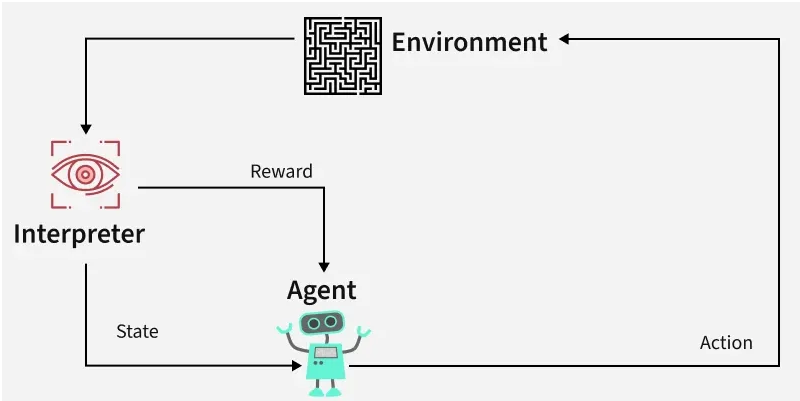
\includegraphics[width=0.8\textwidth]{Images/Chapter1/reinforcement.png}
  \caption{Illustration of the Reinforcement learning process \cite{geeksforgeeks2025supervised} }
  \label{fig:reinforcement}
\end{figure}


\section{Deep Learning}
\label{sec:dl}
Deep learning has emerged as a powerful approach for modeling complex data through architectures that incorporate non-linear transformations. Neural networks, including deep neural networks, serve as the fundamental components of deep learning. These techniques have achieved remarkable progress in various domains such as sound and image processing, enabling tasks like facial recognition, speech recognition, computer vision, language processing, and text classification. The potential applications of deep learning are vast and continue to expand.

Different types of neural network architectures, such as multilayer perceptrons, Convolutional Neural Networks (\glsxtrshort{cnn}s), and recurrent neural networks, cater to specific data types and tasks. These architectures are characterized by deep layers organized in a cascading manner.

\begin{figure}[H]
  \centering
  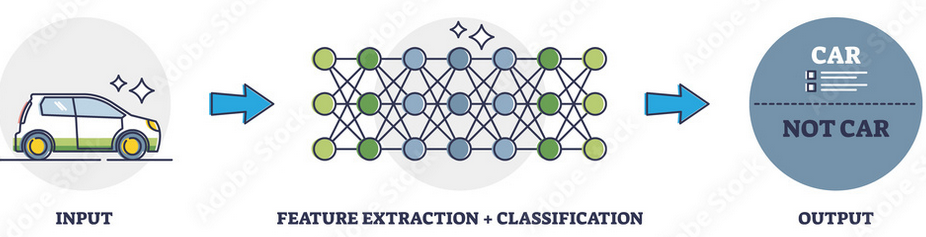
\includegraphics[width=0.8\textwidth]{Images/Chapter1/dl.png}
  \caption{Illustration of the Deep Learning Process. \cite{alltius2025deeplearning}}
  \label{fig:dl}
\end{figure}

% \subsection{History of Deep Learning}
% \label{sec:dl_history}
% The history of deep learning spans several decades, with key developments occurring in distinct waves of innovation. The foundational concept of artificial neural networks dates back to 1943 when Warren McCulloch and Walter Pitts proposed a computational model of neurons \cite{mcculloch1943logical}. The field progressed with Frank Rosenblatt's introduction of the perceptron in the late 1950s, which demonstrated the ability to perform simple pattern recognition \cite{rosenblatt1958perceptron}.

% However, the field faced significant challenges in the 1970s after Marvin Minsky and Seymour Papert published "Perceptrons" \cite{minsky1969perceptrons}, highlighting the limitations of single-layer neural networks. This initiated what is now known as the "AI winter," a period of reduced funding and interest in neural network research.

% The 1980s saw a resurgence with the development of backpropagation by Geoffrey Hinton, David Rumelhart, and Ronald Williams \cite{rumelhart1986learning}, enabling effective training of multi-layer networks. However, computational limitations prevented widespread adoption of deeper architectures.

% The modern era of deep learning began in the 2000s with several breakthrough developments:
% \begin{itemize}
%   \item In 2006, Geoffrey Hinton introduced deep belief networks with an effective layer-by-layer pre-training method \cite{hinton2006fast}.
%   \item In 2012, AlexNet, developed by Alex Krizhevsky, Ilya Sutskever, and Geoffrey Hinton, dramatically outperformed traditional computer vision algorithms in the ImageNet competition \cite{krizhevsky2012imagenet}.
%   \item Subsequent years saw the development of increasingly sophisticated architectures such as VGGNet, GoogLeNet/Inception, and ResNet, each advancing the state-of-the-art in various tasks.
% \end{itemize}

% In the medical imaging domain, a significant milestone was the introduction of U-Net in 2015 by Ronneberger et al. \cite{ronneberger2015unet}, specifically designed for biomedical image segmentation, demonstrating deep learning's capacity to address specialized healthcare challenges.

\subsection{Why Deep Learning?}
\label{sec:why_dl}

Deep learning offers several distinct advantages that have fueled its adoption across numerous domains, particularly in medical imaging:

\begin{itemize}
  \item \textbf{Automatic Feature Extraction}: Unlike traditional machine learning that relies on handcrafted features, deep learning automatically discovers relevant features from raw data, eliminating the need for domain-specific expertise in feature engineering \cite{shen2017deep}.

  \item \textbf{Hierarchical Feature Learning}: Deep networks learn representations at multiple levels of abstraction. Lower layers capture basic patterns (e.g., edges in images), while higher layers combine these to represent complex concepts (e.g., textures, objects, or tumor characteristics) \cite{shen2017deep}.

  \item \textbf{Scalability with Data}: Deep learning models continue to improve as more data becomes available, unlike many traditional algorithms that plateau in performance. This is particularly relevant in medical imaging as dataset sizes continue to grow \cite{shen2017deep}.

  \item \textbf{Transfer Learning}: Knowledge gained from one task can be transferred to another, reducing the need for large amounts of labeled data for each new application—crucial in medical domains where annotated data is often scarce \cite{tajbakhsh2016convolutional}.

  \item \textbf{End-to-End Learning}: Deep learning can learn directly from raw input to desired output, eliminating intermediate processing steps that might introduce biases or errors \cite{nguyen2020end}.

  \item \textbf{Handling Unstructured Data}: Medical images, natural language reports, and other unstructured data that constitute most healthcare data are particularly well-suited for deep learning approaches \cite{shen2017deep}.
\end{itemize}

% \subsection{Deep Learning Application Examples}
% \label{sec:dl_applications}
% Deep learning has revolutionized numerous fields with successful applications across diverse domains:

% \begin{itemize}
%   \item Retinal disease detection from optical coherence tomography
%   \item Lung cancer detection and classification from CT scans
%   \item Skin lesion classification for melanoma detection
%   \item Breast cancer detection in mammography
%   \item Object detection and recognition in images and video
%   \item Facial recognition and emotion detection
%   \item Sentiment analysis in social media and customer feedback
%   \item Text summarization and content generation
%   \item Speech recognition and transcription
% \end{itemize}

These few mentioned examples illustrate deep learning's versatility and transformative impact across domains.

\subsection{Different Architectures of Deep Learning}
\label{sec:dl_architectures}
Deep learning encompasses a variety of architectural paradigms, each designed to address specific types of problems:

\textbf{Feedforward Neural Networks (FNNs)}:
The most basic architecture where information flows only in one direction, from input to output. Multilayer Perceptrons (MLPs) are a common type of FNN with multiple hidden layers, suitable for tabular data and basic pattern recognition tasks.

\textbf{Convolutional Neural Networks (CNNs)}:
Specialized for processing grid-like data such as images. CNNs employ convolutional layers that apply filters across the input, capturing spatial hierarchies and patterns. Notable CNN architectures include:
\begin{itemize}
  \item \textbf{AlexNet}: Pioneering architecture that demonstrated the power of deep learning in computer vision \cite{krizhevsky2012imagenet}
  \item \textbf{VGGNet}: Featured uniform architecture with small filters \cite{simonyan2014very}
  \item \textbf{ResNet}: Introduced residual connections to train very deep networks effectively \cite{he2016deep}
  \item \textbf{Inception/GoogLeNet}: Employed multi-scale processing through parallel convolutional filters \cite{szegedy2015going}
  \item \textbf{DenseNet}: Connected each layer to every other layer in a feed-forward fashion \cite{huang2017densely}
  \item \textbf{U-Net}: Specialized for biomedical image segmentation with a contracting path and an expansive path \cite{ronneberger2015unet}
\end{itemize}

\textbf{Recurrent Neural Networks (RNNs)}:
Designed for sequential data by maintaining internal memory states. Variants include:
\begin{itemize}
  \item \textbf{Long Short-Term Memory (LSTM)}: Addresses the vanishing gradient problem with specialized memory cells \cite{hochreiter1997long}
  \item \textbf{Gated Recurrent Units (GRU)}: Simplified version of LSTM with fewer parameters \cite{cho2014learning}
  \item \textbf{Bidirectional RNNs}: Process sequences in both forward and backward directions
\end{itemize}

\textbf{Transformer Networks}:
Introduced in the paper "Attention Is All You Need" \cite{vaswani2017attention}, transformers rely on self-attention mechanisms rather than recurrence or convolution. They have revolutionized NLP through models like BERT, GPT, and T5, and are increasingly applied to computer vision tasks.

\textbf{Generative Models}:
\begin{itemize}
  \item \textbf{Generative Adversarial Networks (GANs)}: Consist of generator and discriminator networks trained simultaneously in a minimax game \cite{goodfellow2014generative}
  \item \textbf{Variational Autoencoders (VAEs)}: Encode inputs to a latent space distribution and decode samples from this distribution \cite{kingma2013auto}
  \item \textbf{Diffusion Models}: Generate data by gradually removing noise from a signal \cite{ho2020denoising}
\end{itemize}

\textbf{Hybrid Architectures}:
Many modern deep learning solutions combine elements from different architectural paradigms to leverage their respective strengths. For example, CNN-LSTM networks for video analysis or attention-augmented CNNs for improved image recognition.

\subsection{Convolutional Neural Networks (CNNs)}
\label{sec:cnn}
A convolutional neural network (CNN) is a type of neural network with a topology similar to a grid, inspired by the human brain. It is commonly used for image processing tasks, as well as natural language processing.

A CNN consists of two main parts. The input is an image, represented as a 2D matrix of pixels for grayscale images and a 3D matrix of pixels for color images (Red, Green, Blue).

The first part of a CNN is the convolutional layer, which acts as a feature extractor. The image is passed through a series of filters, or convolution kernels, to generate new images called feature maps. Some intermediate filters reduce the image resolution. Finally, the feature maps are concatenated to form a vector of features, known as the CNN code.

The output of the convolutional layer, the CNN code, is the input to the second part of the network. The main role of this part is to combine the features of the CNN code to classify the image. The output is a final layer with one neuron per category.
\begin{figure}[H]
  \centering
  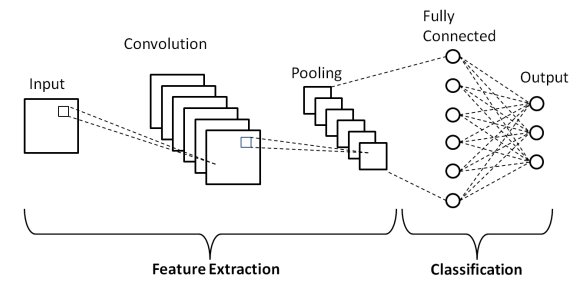
\includegraphics[width=0.8\textwidth]{Images/Chapter1/cnn.png}
  \caption{Convolutional Neural Network Architecture \cite{phung2019high}}
  \label{fig:cnn}
\end{figure}

\subsubsection{Convolutional Layer}
\label{sec:conv}

The convolutional layer is the most important layer and usually the first layer in a CNN. It takes an image and a filter as input and applies the convolution operation to produce a new image, called the activation map or feature map.

The activation map values are calculated using the following formula:
\begin{equation}
  G[m,n] \;=\; (f * h)[m,n]
\end{equation}
where
\begin{itemize}
  \item $f$ is the input image,
  \item $h$ is the convolution filter,
  \item $m,n$ are the spatial indices over which the convolution is computed.

\end{itemize}
\begin{figure}[H]
  \centering
  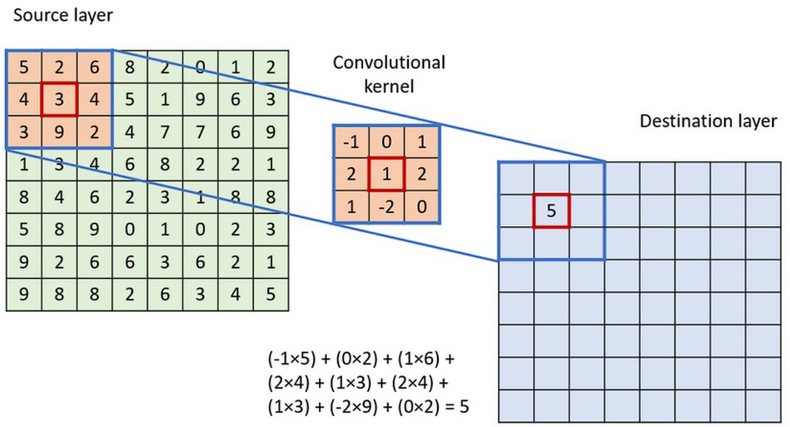
\includegraphics[width=0.6\textwidth]{Images/Chapter1/conv.png}
  \caption{Convolution Layer in a Convolutional Neural Network \cite{oulmi2018classification}}
  \label{fig:conv}
\end{figure}

\subsubsection{Correction Layer (ReLU)}

The Correction Layer, typically implemented using the Rectified Linear Unit (ReLU), is an activation function applied after each convolution operation to enhance processing efficiency. It replaces all negative pixel values with zero, introducing non-linearity into the network while maintaining computational simplicity. The ReLU function is defined as:

\begin{equation}
  f(x) = \max(0, x)
\end{equation}

Several other activation functions exist, such as the sigmoid function, the hyperbolic tangent function (tanh), and the hyperbolic saturating tangent function. However, ReLU is often preferred in deep learning models because it enables faster convergence and better performance compared to these alternatives.

\subsubsection{Pooling Layers}

Pooling layers are utilized to reduce the spatial dimensions of feature maps while preserving the most important information and features. This helps decrease computational complexity and mitigate overfitting. There are several types of pooling operations:

\begin{itemize}
  \item \textbf{Max Pooling}:
        It selects the maximum value from each patch of the feature map. Typically, a $2 \times 2$ patch is used. Max pooling is the most commonly used pooling method.

  \item \textbf{Min Pooling}:
        The inverse of max pooling; it selects the minimum value from each patch of the feature map.

  \item \textbf{Average Pooling}:
        It computes the average of all the values within each patch of the feature map by summing the values and dividing by the number of elements.

  \item \textbf{Sum Pooling}:
        It computes the sum of all elements within each patch of the feature map.

  \item \textbf{Flattening}:
        After the pooling operations, the resulting feature maps are flattened into a single one-dimensional vector to prepare for fully connected (dense) layers.
\end{itemize}

\subsubsection{Fully Connected Layer}

After the convolution and pooling layers, the high-level reasoning in the neural network is done in fully connected layers. The output of flattening is the input of fully-connected layers which are the same as artificial neural networks and carry out the same mathematical operations. The last fully-connected layer uses an activation function such as sigmoid or softmax to get probabilities of the outputs.



\section{Conclusion}
\label{sec:conclusion}

In this chapter, we established the core concepts and distinctions between AI, machine learning, and deep learning, reviewed key algorithms and architectures—from SVMs and decision forests to CNNs, transformers, and U‑Nets—and illustrated how these methods enable robust pattern recognition, automated analysis, and end‑to‑end learning on complex medical imaging data; this theoretical foundation directly supports our subsequent work on brain tumor segmentation and classification, where we will detail data preprocessing, the U‑Net implementation, and model evaluation against clinical standards.
